
\section{Name und Begleitfiguren}\label{}

Das Projekt hei"st ``Mumie''\footnote{Aktuell bem"uhen wir uns, die
domain zu erwerben...}.

Es gibt \textbf{zwei} Begleitfiguren:

\begin{list_sabina}
\item
\textbf{Mumie}:\\
Die Mumie ist der ``Hauptcharakter''.
Sie unterst"utzt den User  mit Schwerpunkt auf den \textit{fachlichen} Hinweisen.
\item
\textbf{Skarab"aus}:\\
Der Skarab"aus ist Partner der Mumie (etwa bei Dialogen), er
unterst"utzt au"serdem den User mit Schwerpunkt auf den 
\textit{organisatorischen} Anweisungen.
\end{list_sabina}


\begin{figure}[h]
\begin{center}
\ifx\pdfoutput\undefined
  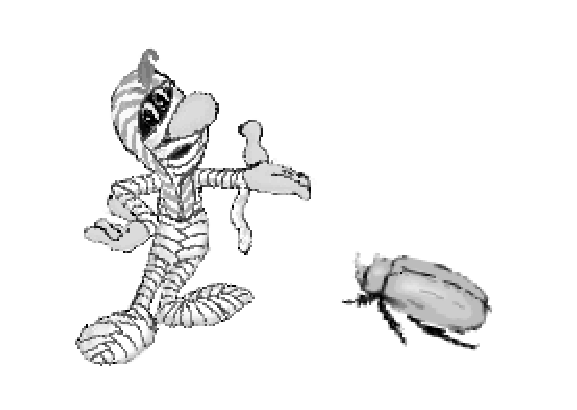
\epsfig{file=Skizzen/my_combi_02.eps, height = 5cm}
\else
  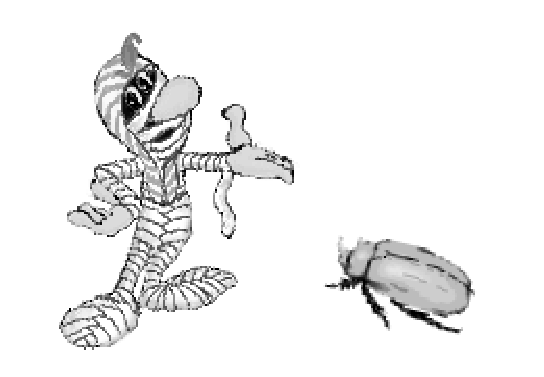
\includegraphics{Skizzen/my_combi_02.pdf}
\fi
\caption{Die Begleitfiguren (nur ``funktionale Skizze'')}
\end{center}
\end{figure}


Die Eins"atze der Begleitfiguren sind toolspezifisch und werden 
daher jeweils in den entsprechenden Tools beschrieben.


\vspace{10mm}

{\footnotesize\textit{Ideen/Layoutvorschl"age: Die Figuren sollten
comicartige Figuren sein und in verschiedenen Ausf"uhrungen (sitzend,
stehend, mit Buch in der Hand, auf fliegendem Teppich, ...), mit
verschiedener Gestik/Mimik (lachend, irristiert, sich die Haare
raufend, ...) und animiert verwenden werden k"onnen. Die Mumie
k"onnte etwa Miraculix oder auch Gandalf nachempfungen sein... weise,
aber auch viel Charakter. Eingewickelt nat"urlich. Der Skarab"aus
k"onnte sich an Kassiopeia (Michael Ende, Momos Schildkr"ote)
anlehnen: die hatte bisweilen eine Leuchtschrift auf dem R"ucken...}}
